\subsection{Polarization Leakage from Detector Array}

\paragraph{Description:}

Beam asymmetries from the optical coupling to the array can cause leakage from temperature to polarization and E-modes to B-modes. The beams need to be modeled and measured so that they can be correctly incorporated into the analysis to minimize these effects.

\paragraph{Plan to model and/or measure:}
The simplest way to model this effect is by assuming a pair-differenced detector. In the case that a HWP is used, this effect is mitigated because there is no pair differencing. To estimate this effect with a HWP, one would have to propagate the analysis through a demodulated timestream, but this method is still useful in this case because it can give an upper limit on the effect. In the non-HWP case, the polarization angle of the detector can be used instead of pair-differencing to determine the polarized signal.

The polarization leakages in the power spectra are estimated using the simulated co- and cross-polar beams from HFSS. Assuming a pair-differenced detector, the electric fields on the sky $E_x$ and $E_y$ are coupled to the electric field in the detectors $E_a$ and $E_b$ by
\begin{equation}\label{eqn:beams}
  \begin{bmatrix}
  E_a\\
  E_b
  \end{bmatrix}
  =
  \begin{bmatrix}
  \beta_{ax} & \beta_{ay}\\
  \beta_{bx} & \beta_{by}
  \end{bmatrix}
  \begin{bmatrix}
  E_x\\
  E_y
  \end{bmatrix}
  \,\,\, ,
\end{equation}
where $a$ and $x$ as well as $b$ and $y$ are aligned along the boresight. Here $\beta_{ax}$ and $\beta_{by}$ are the co-polar beams, and $\beta_{ay}$ and $\beta_{bx}$ are the cross-polar beams. The default setting in HFSS is to source the calculation through the wave port in the $x$ direction, which gives $\beta_{ax}$ and $\beta_{ay}$. To model $\beta_{bx}$ and $\beta_{by}$, the source must be changed to the wave port in the $y$ direction. The complex beams are then given by the sum of their real and imaginary parts as
\begin{align}
\beta_{nx} & =  \mathrm{Re}(rEL3X)+i\, \mathrm{Im}(rEL3X) \nonumber \\
\beta_{ny} & =  \mathrm{Re}(rEL3Y)+i\, \mathrm{Im}(rEL3Y)\,\,\,\,\,,
\end{align}
where $n$ is either $a$ or $b$. The co- and cross-polar beams from HFSS are then masked such that they go to zero outside of the Lyot stop, and a 2D FFT is performed to estimate the far field beams~\cite{Simon_Thesis_2016}.

For an ideal bolometer differencing pair at the output of the of the horn, the measured polarized signal $P$ would be
\begin{equation}\label{eqn:p1}
P=E_a-E_b \,\,\,\,.
\end{equation}
The Stokes parameters using the decreasing phase convention are given by
\begin{align}\label{eqn:Stokes}
I & =  |E_{x}|^2+ |E_{y}|^2  \nonumber \\
Q & =   |E_{x}|^2- |E_{y}|^2  \nonumber \\
U & =  2\,\mathrm{Re}(E_{x} E_{y}^{*}) \nonumber \\
V & =  2\,\mathrm{Im}(E_{x} E_{y}^{*})\,\,\,\,\,.
\end{align}
Here $I$ is the intensity, $Q$ and $U$ describe the linear polarization, and $V$ describes the circular polarization. Substituting Equation~\ref{eqn:beams} into Equation~\ref{eqn:p1} and using the definition of the Stokes parameters  as in Equation~\ref{eqn:Stokes} gives
\begin{equation}
P=\sigma I + \delta Q + \epsilon U+ \gamma V\,\,\,\, ,
\end{equation}
where the coefficients are the beam couplings from $I$, $Q$, $U$, and $V$ into $P$. For an ideal detector, $\delta=1$ and $\sigma=\epsilon=\gamma=0$. The beam couplings are then given by
\begin{align}\label{eqn:leakage beams}
\sigma & =  \frac{1}{2} (\beta_{ax}^2 + \beta_{ay}^2 - \beta_{bx}^2 - \beta_{by}^2) \\
\delta & =   \frac{1}{2} (\beta_{ax}^2 - \beta_{ay}^2 - \beta_{bx}^2 + \beta_{by}^2) \\
\epsilon & =  \mathrm{Re}(\beta_{ax}^{*} \beta_{ay} - \beta_{bx}\beta_{by}^{*} )  \\
\gamma & =  -\mathrm{Im}(\beta_{ax} \beta_{ay}^{*} + \beta_{bx}^{*}\beta_{by} )\,\,\,\,\,.
\end{align}
The beams are then normalized by the maximum of $\delta$ and averaged across each observation band. A more sophisticated analysis could weight the frequency average by the total bandpass. As the distance from the center of the array increases, the ellipticity of the Lyot stop as viewed from the pixel increases, which results in higher leakage. The central pixel thus gives the lowest temperature to polarization leakage. While edge pixels exhibit higher leakage, the average leakage beam of pairs of pixels equidistant from the array center on opposite sides of the array approximates the behavior of the central pixel. Therefore, the behavior of the central pixel can provide an estimate for the systematics of the array~\cite{Simon_Thesis_2016}.

We estimate the leakage in the power spectra from these band-averaged beams with two methods: a map-based systematics pipeline and a window function method. The map-based method gives a full estimation of this effect using the leakage beams and simulated maps and realistic noise estimates. This method is useful for determining how much of the temperature to polarization leakage goes into E-modes versus B-modes. With the window function method, the leakage is estimated using the calculated window functions of the signal and leakage beams. This simplified model is quick to model, but only gives total polarization leakage versus how much of the leakage goes into E-modes versus B-modes. However, it is still good as a check on the worst-case scenario. For feedhorns, the main source of the leakage is from ellipticity. Based on symmetry arguments presented in Shimon et al., 2008~\cite{Shimon_2008}, the temperature to polarization leakage goes largely into E-modes, and the E-mode to B-mode leakage is negligible. Simulations from the map-based pipeline also show that this is the case. Because of the wobble effect in a sinuous antenna coupled to a lenslet, the temperature to polarization leakage has a large contribution to the B-modes, and the E-mode to B-mode leakage is large.

In the window function method, for each beam, the magnitude squared of the FFT of the averaged far field beams is calculated and normalized by the maximum of the transformed $\delta$ beam. Next the 2D functions are binned radially to make a 1D window function. To account for the rest of the telescope optics, the multipole axis is noramlized by the telescope beam size either from full telescope optics simulations or by calculating the beam size at the center frequency of the observation band assuing a diffraction-limited beam. The measured spectra are then estimated by multiplying simulations of the EE and BB polarization spectra by the $\delta$ window function, the temperature to polarization leakage spectrum is determined by multiplying the simulated TT spectrum by the $\sigma$ window function, and the EE to BB leakage is determined by multiplying the simulated EE spectrum by the $\epsilon$ window function. 

In general, as pixel size increases, the feedhorn optimization has more aperture to work with, so the systematics level decreases in both bands. The decrease in the lower band is usually smaller because the waveguide cutoff of the horn can cause beam distortion. This effect can be modeled more precisely with the full bandpass weighted beam average. Feedhorns are also tunable in their design based on the penalty function used for optimization, so if the systematics levels are ever too high for a given design, the horn optimization can sacrifice beam coupling efficiency for better symmetry and vice versa. For the sinuous and lenslet case, as pixel size increases, there is no overall decrease in the level of systematics. Instead, as the pixel size increases, the level of leakage in the high band increases, while the level of the leakage decreases in the low band and vice versa.

Cross-linking in the maps can help identify and quantify this leakage. Accounting for beam asymmetries in the analysis can mitigate the leakage by an order of magnitude or more. The level of this mitigation is dependent on how well the telescope beams are characterized by planets, point sources, and/or calibration sources. Prior to deployment, we can use beam measurements from a warm vector network analyzer and cold beams in lab to characterize the detector array beams isolated from the rest of the optics. Additional mitigation is needed both in the design of the arrays and the analysis for the lenslet and sinuous detector arrays since mitigating the wobble effects necessitates the use of the four-pixel subtraction scheme. In the SAC, the use of HWPs is expected to mitigate this effect by a factor greater than 10.


\paragraph{Uncertainty/Range:}
Ideally, any leakage into the polarized spectra should be lower than the B-mode signal by several orders of magnitude. The EE to BB leakage is negligible for the feedhorn in both the LAT and SAC cases. For the lenslet and sinuous detector, the EE to BB leakage is at the level of the B-modes without any mitigation for both the LAT and SAC cases. Window-function simulations for the LAT, show that the total polarization leakage is several orders of magnitude below the B-mode signal for both the feedhorn and lenslet architectures. For the SAC, which has a larger stop, the level of the temperature to poalrization leakage is comparable to the level of the B-modes so the full map-based pipeline must be employed. Using this method, it can be determined that the feedhorn and lenslet architectures both have acceptable levels of leakage (when only the wobble mitigation for the lenslet is included). However, it is also imporatant to note that the SAC will have a HWP, which will strongly mitigate this effect. Some examples of the leakage estimation using the window function method for preliminary SO designs at a 5.3~mm pixel size on the LAT are shown in Figures~\ref{fig:MF_90_TP_leakage}-\ref{fig:MF_150_EB_leakage}.

\begin{figure}[h!]
\centering
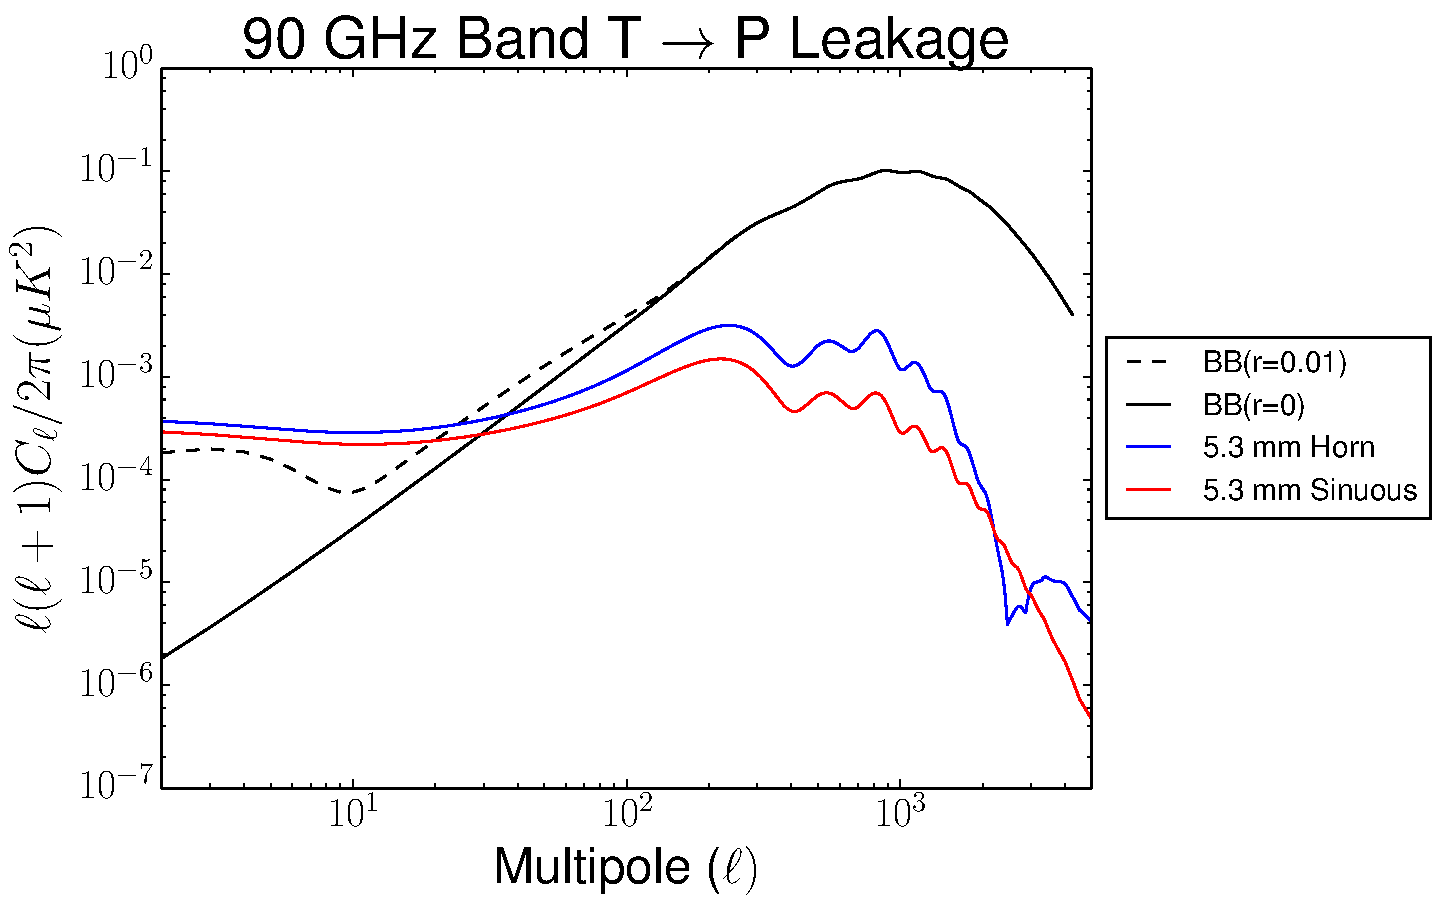
\includegraphics[width=\textwidth]{figures/90GHz_band_ITT_pixel_size_horn_sinuous_5p3mm.pdf}
\caption{The temperature to polarization leakage of the AdvACT spline-profiled feedhorn design (blue) and a lenslet and sinuous design (red) for a 5.3 mm pixel size at 90 GHz. Note that the leakage goes primarily into E-modes for the feedhorn.}
\label{fig:MF_90_TP_leakage}
\end{figure}

\begin{figure}[h!]
\centering
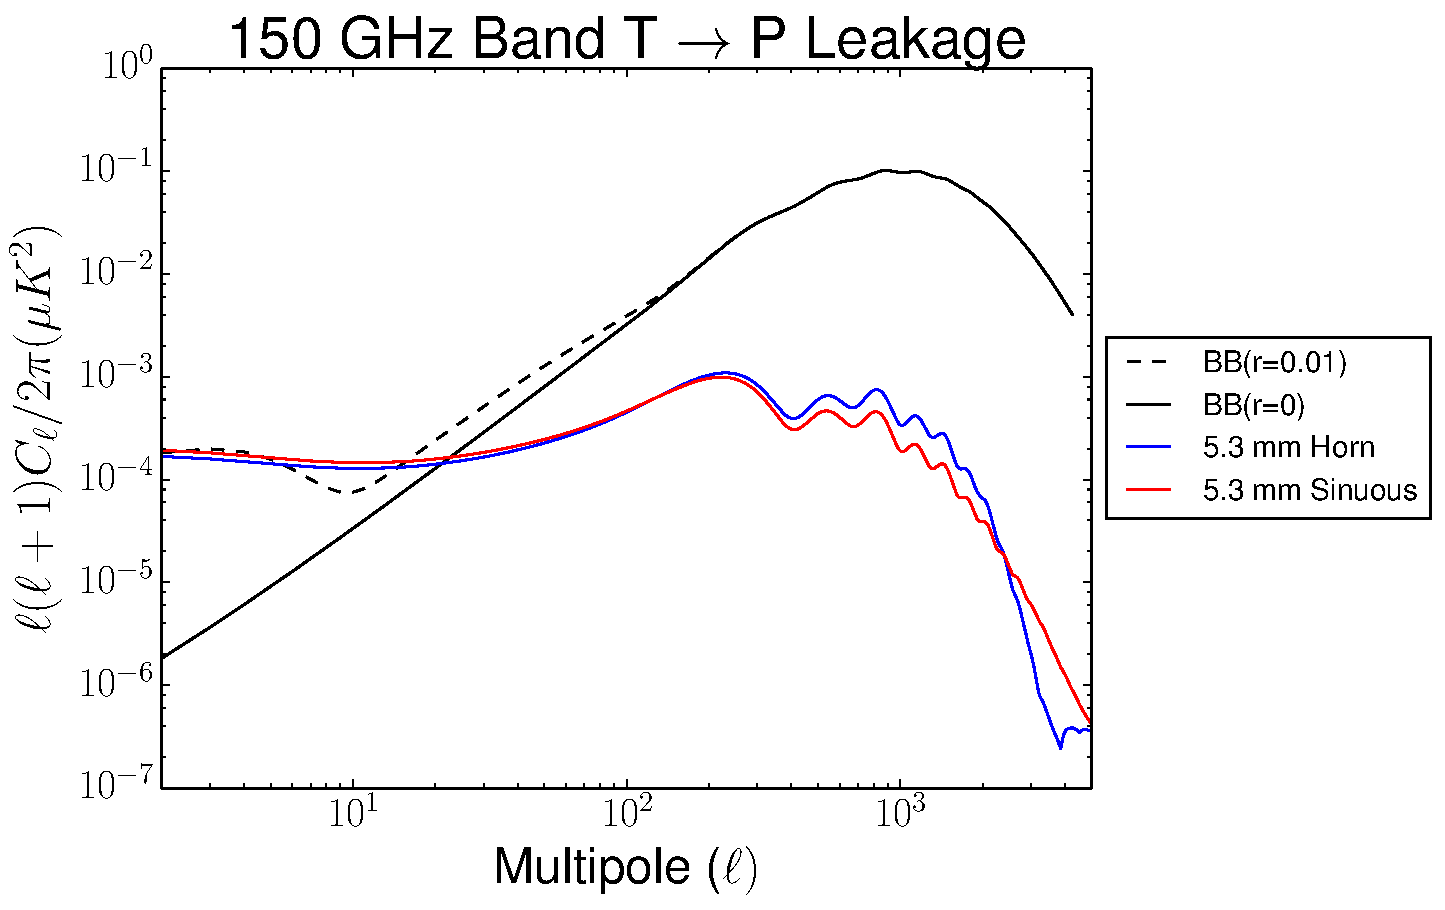
\includegraphics[width=\textwidth]{figures/150GHz_band_ITT_pixel_size_horn_sinuous_5p3mm.pdf}
\caption{The temperature to polarization leakage of the AdvACT spline-profiled feedhorn design (blue) and a lenslet and sinuous design (red) for a 5.3 mm pixel size at 150 GHz. Note that the leakage goes primarily into E-modes for the feedhorn.}
\label{fig:MF_150_TP_leakage}
\end{figure}

\begin{figure}[h!]
\centering
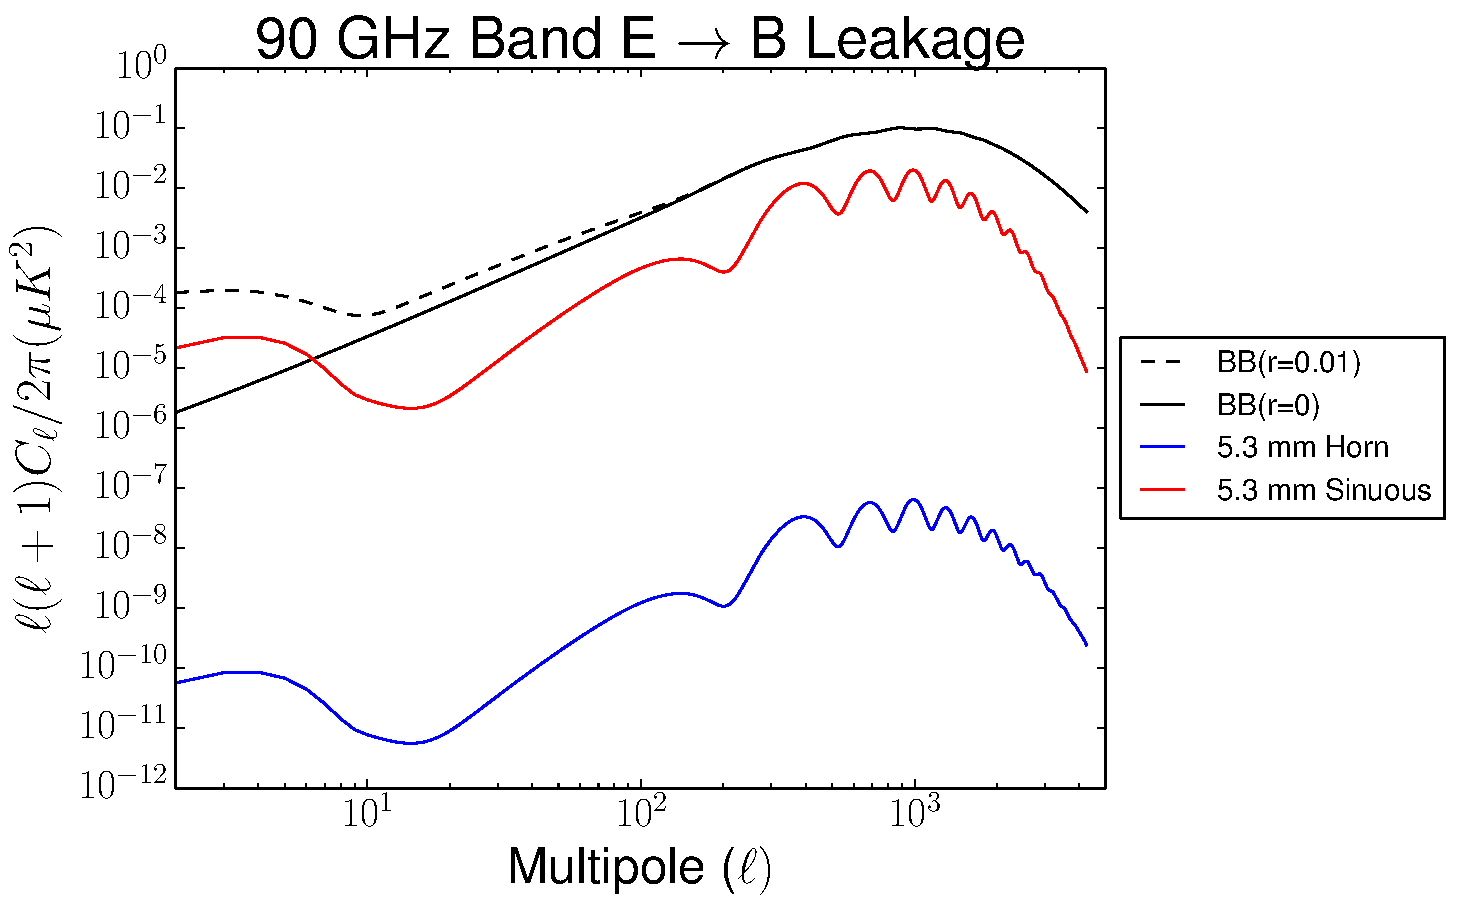
\includegraphics[width=\textwidth]{figures/90GHz_band_UEE_pixel_size_horn_sinuous_5p3mm.pdf}
\caption{The E-mode to B-mode leakage of the AdvACT spline-profiled feedhorn design (blue) and a lenslet and sinuous design (red) for a 5.3 mm pixel size at 90 GHz. Note that the leakage of the feedhorn is negligibly low and that the contribution from the lenslet and sinuous antenna is from the polarization wobble.}
\label{fig:MF_90_EB_leakage}
\end{figure}

\begin{figure}[h!]
\centering
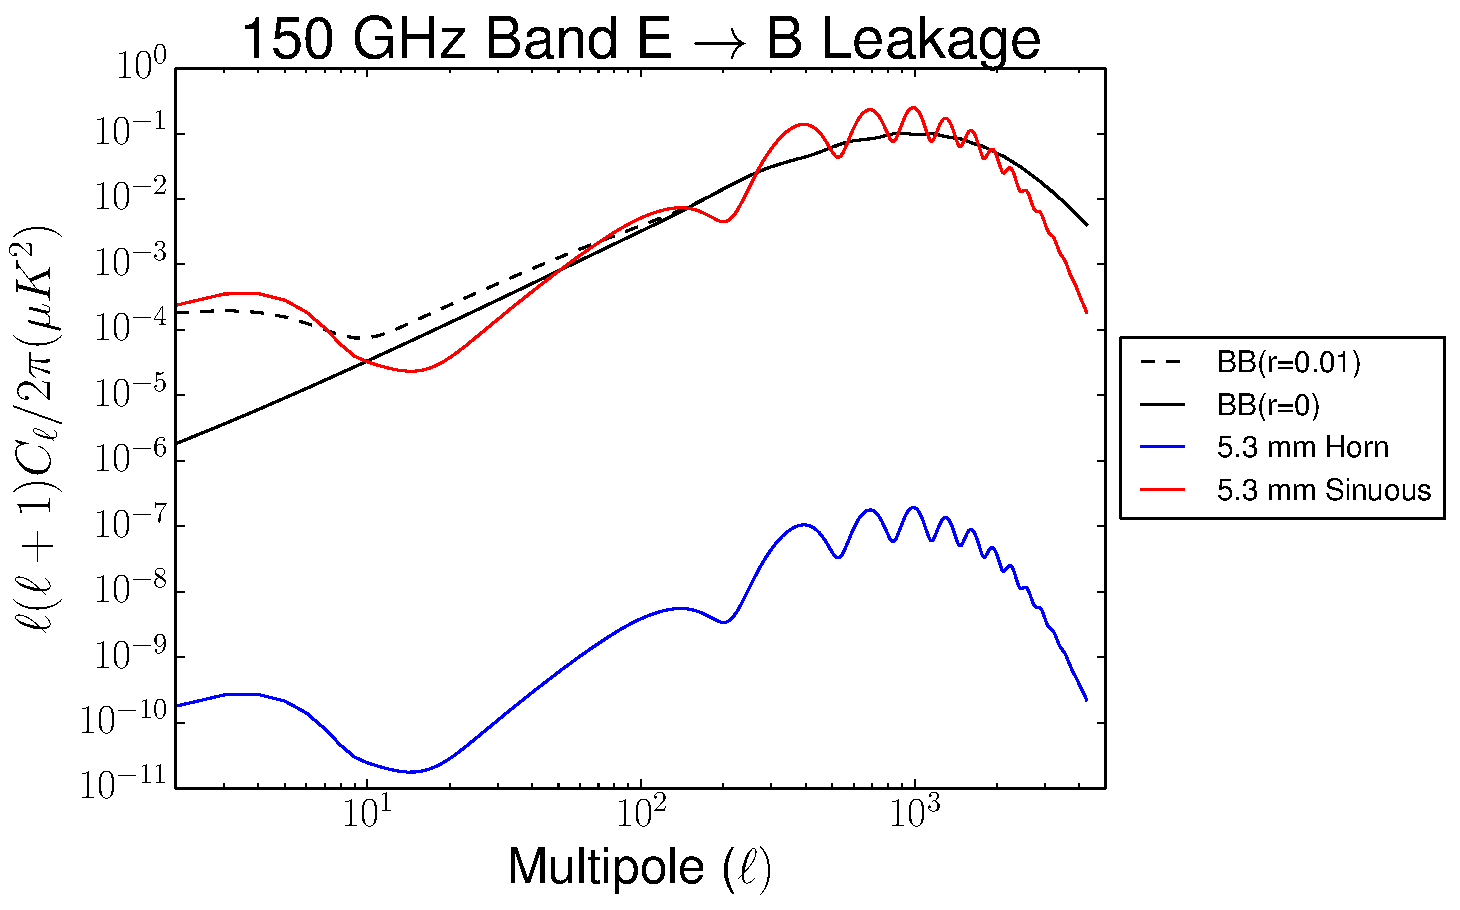
\includegraphics[width=\textwidth]{figures/150GHz_band_UEE_pixel_size_horn_sinuous_5p3mm.pdf}
\caption{The E-mode to B-mode leakage of the AdvACT spline-profiled feedhorn design (blue) and a lenslet and sinuous design (red) for a 5.3 mm pixel size at 150 GHz. Note that the leakage of the feedhorn is negligibly low and that the contribution from the lenslet and sinuous antenna is from the polarization wobble.}
\label{fig:MF_150_EB_leakage}
\end{figure}

\paragraph{Parameterization:}
This can be parameterized with the estimated leakage spectra from the pair-differenced model.

